%% This is an example first chapter.  You should put chapter/appendix that you
%% write into a separate file, and add a line \include{yourfilename} to
%% main.tex, where `yourfilename.tex' is the name of the chapter/appendix file.
%% You can process specific files by typing their names in at the 
%% \files=
%% prompt when you run the file main.tex through LaTeX.
% \let\chaptername\relax
\renewcommand\chaptername{}
\chapter{INTRODUCTION}

Forests are important part of the world's natural ecosystem, maintaining sustainability in terms of economy and ecology in different scales: both locally and globally. 
Exploitation of the forest resources, forest fires and further other reasons lead to deforestation, and this is a common problem at different parts of the world. Russia is no exception here, up to 50\% of its territory is covered by  forest, which makes up more than 20\% of the World’s forestry resources (Figure \ref{Russ}). Moreover, Russia is amongst the top 5 wood exporters, the industry exports are booming in the last decade, and ongoing investments will keep raising output \cite{Taylor2018, Taylor2020, Wwf2007}. Considering the aforementioned facts, it is obvious that efficient management of the forest sector should be established for sustainable and innovative development of forest use, conservation, and reproduction.

\begin{figure}[ht]
\centering
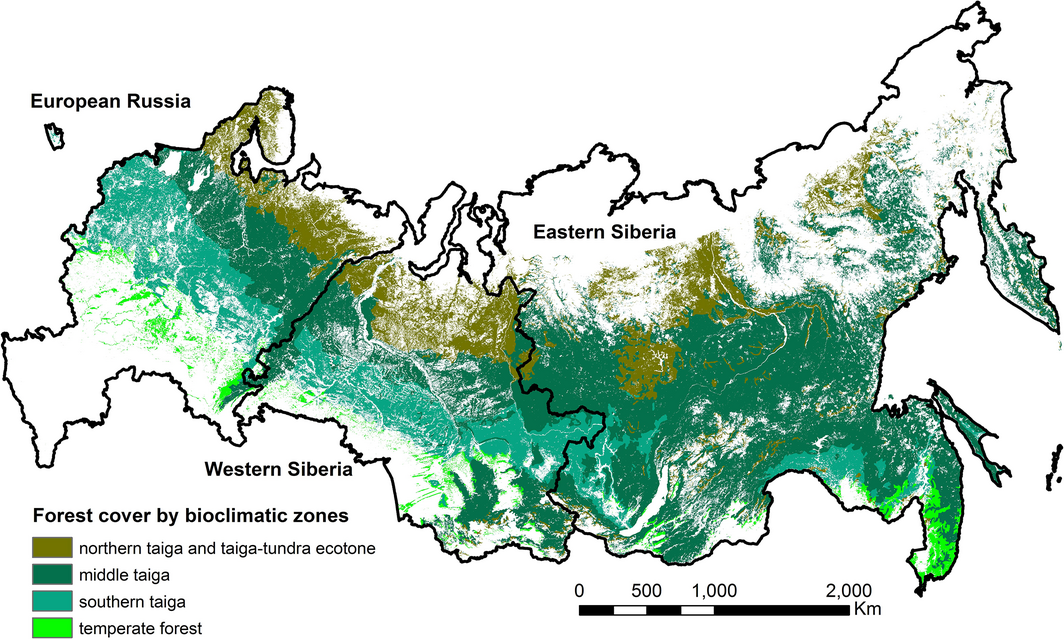
\includegraphics[scale=0.4]{images/RussiaForestCover.png}
\caption{Distribution of forest cover across Russia \cite{Loboda2017}}
\label{Russ}
\end{figure}

Systematic collection of forest information is one of the main tools in effective forest management. Collection of forest information, such as tree counting, tree height and location, species classification, and damage area mapping allows governments to perform statistical analysis to understand the state and dynamics for future planning.

While in-situ field assessment is a good option to obtain comprehensive information about small forest patches, it is still very inefficient method in terms of cost, time and assessment frequency. On the other hand, emerging remote sensing technologies demonstrated a big potential in different fields, such as precision agriculture, land cover changes detection, urban environment monitoring, etc. It can also be beneficial in forest inventory tasks, transforming the scale, price and speed of forestry assessments. High-resolution remote sensing imagery is becoming one of the most extensively used data types in forestry analysis \cite{Tianyang2018}. Nowadays, there are a lot of satellites, which can obtain sub-meter resolution imagery with limited number of spectral bands (Table \ref{table1}) \cite{Gomes2016}. Combined with artificial intelligence remote sensing data can be applied to more challenging problems, since neural networks allows to extract non-trivial features and patterns from the satellite or aerial imagery. 

\begin{table}
\caption{High resolution satellites, their spectral resolution and bands}
\label{table1}
\vskip 0.15in
\begin{center}
\begin{small}
\begin{sc}
\begin{tabular}{l{3cm}p{2cm}p{2cm}p{2cm}p{3cm}}
\hline
\textbf{Satellite} & \textbf{Launch year} & \textbf{Panchromatic resolution (m)} & \textbf{Multispectral resolution (m)}& \textbf{Bands}\\\hline
GeoEye1 &2008  & 0.46 & 1.84 & RGB-\gls{NIR}\\\hline
WorldView2 &2009  & 0.46 & 1.85 & RGB-NIR, RedEdge, Coastal, Yellow, NIR2\\\hline
Pleiades1A &2011  & 0.5 & 2.0 & RGB-NIR\\\hline
Pleiades1B &2012  & 0.5 & 2.0 & RGB-NIR\\\hline
Kompsat-3 &2012  & 0.7 & 2.8 & RGB-NIR\\\hline
SkySat1 &2013  & 0.9 & 2.0 & RGB-NIR\\\hline
SkySat2 &2014  & 0.9 & 2.0 & RGB-NIR\\\hline
WorldView3 &2014  & 0.31 & 1.24 & RGB-NIR, RedEdge, Coastal, Yellow, NIR2\\\hline
Kompsat3A &2015  & 0.55 & 2.2 & RGB-NIR\\\hline
WorldView4 &2016  & 0.34 & 1.36 & Not available\\\hline
\end{tabular}
\end{sc}
\end{small}
\end{center}
\vskip -0.1in
\end{table}

The goal of this research is to develop a pipeline for Individual Tree Crown (\gls{ITC}) detection and delineation from RGB satellite imagery using the processed aerial data for training. The hypothesis is to check that rescaled high-resolution aerial imagery and satellite imagery will have similar domains for the neural network, thereby we will confirm that state-of-the-art Convolutional Neural Network (\gls{CNN}) trained on rescaled aerial RGB imagery is able to delineate the tree crowns directly from the real satellite RGB imagery. We will try to confirm the applicability of the proposed methodology, demonstrate its practical usage for forest inventory to substitute manual tree delineation. For this purpose, the existing methods for automatic tree delineation are to be analyzed, the new dataset will be created and used in the experiments by the following framework. First of all, UAV-carried aerial imagery from Ust-Ilimsk region (Irkutsk oblast, Russia) was processed to obtain the high resolution orthophotos and Digital Elevation Models (\gls{DEM}) files. Applying different morphological operations and algorithms on generated data ground truth masks of \gls{ITC} were created for the Regions of Interest (\gls{ROI}). After that, the aerial orthophotos and ground truth masks are to be rescaled to two different satellite resolutions (namely 0.5m and 0.31m, which correspond to WV-2 and WV-3 satellite resolutions respectively) to imitate the satellite imagery. Two independent experiments were performed on these different spatial resolution datasets. The data was used for training the \gls{CNN} to delineate individual trees, and then validated on a separate part of the dataset and several manually delineated satellite images. Overall, remote sensing and deep learning-based framework for \gls{ITC} was built and validated. Results, obtained from the experiments, confirm the feasibility of the proposed approach. Also, the limitations and challenges were described, and possible developments pathways are discussed in the further sections of this research. 

The first part of this work describes essential notions and previously performed research in forest inventory. The second part of the thesis describes obtained data and the proposed methodology. The description and architecture of the deep neural network used in this research is presented in the chapter. The final part presents the results, discussion of findings, limitations, and possible applications.